\section{Results and Discussion}
In order to compare several methods (architecture, feature selection), we train on the ABIDE dataset
with a systematic method proposed below.

First, we split the dataset into a training (90\%), validation (10\%) a test set (10\%).
Then, we train the model on the training set and evaluate the model on the test set.

\subsection{Result of DenseNN on original features}

\begin{figure}[h!]
    \centering
    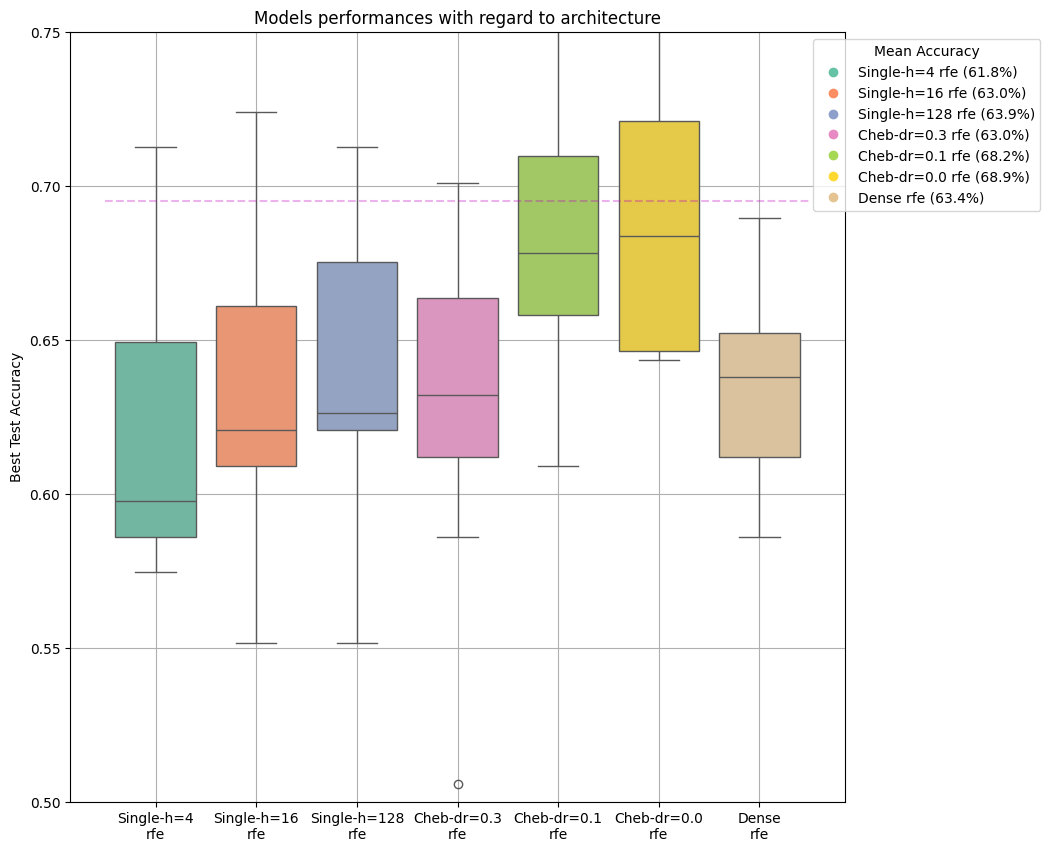
\includegraphics[width=0.45\textwidth]{figures/model_performances_architecture.png}
    \caption{Classification accuracy: comparison of different architectures.
    Single architectures are composed of a single hidden layer with a given number of neurons $h$.
    \textit{Dense} architecture refer to a fully connected neural network with a single hidden layer.
    \textit{Cheb} architectures refer to the graph convolution architecture, we vary the dropout rate $dr$
    during training.}
    \Description{}
    \label{fig:results_architecture}
\end{figure}

\begin{table}[H]
	\begin{center}
		\begin{tabular}{lll}
			Model & Feature & Test accuracy \\
			\hline
			Single-h=4 & rfe & 61.8 +/- 4.4\% \\
			Single-h=16 & rfe & 63.0 +/- 5.1\% \\
			Single-h=128 & rfe & 63.9 +/- 4.6\% \\
			Cheb-dr=0.3 & rfe & 63.0 +/- 5.4\% \\
			Cheb-dr=0.1 & rfe & 68.2 +/- 4.0\% \\
			Cheb-dr=0.0 & rfe & 68.9 +/- 4.0\% \\
			Dense & rfe & 63.4 +/- 3.3\% \\
		\end{tabular}
	\end{center}
	\caption{Models performances with regard to architecture}
	\label{table:dependance_on_architecture}
\end{table}


\subsection{Result on reduced features}

\subsection{Main limitations}

(example where the method does not work) 